% Proposal for the features and scoring and stuff of my senior project.
\documentclass{article}
\title{Senior Project Presentation}
\author{Steve Jarvis}
\date{\today}
% Disables chapter and section numbering
\setcounter{secnumdepth}{-1} 
\usepackage[pdftex]{graphicx}
\usepackage{listings}

\begin{document}
\maketitle

\section{What I Learned...}
\subsection{What's a Neural Network?}
    \paragraph{}A neural network is a general machine learning tool that can be used to 
    learn a large variety of data sets. A neural network is a set of connected weights,
    and the nodes of the network are activations of the input based on the corresponding
    weights.
    \paragraph{}The simplest neural network is one consisting of two layers. A weight
    connects each node in the first layer to each node in the second layer. For example,
    the following diagram could represent a two-layer network used to learn the OR logic
    gate. Imagine three input nodes and two output, with the bottom left representing false
    and the bottom right true. When inputting bits representing logical OR, the network
    should yield output representing true. See Figure~\ref{basicnetwork} on 
    page~\pageref{basicnetwork} for an illustration.
    \begin{figure}
        \centering
        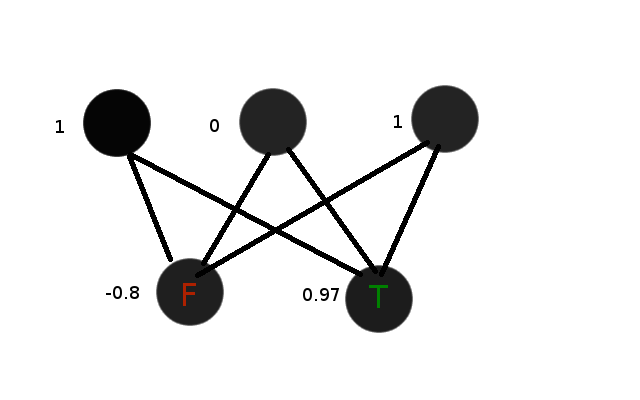
\includegraphics[scale=0.4]{images/perceptron.png}
        \caption{The top layer are inputs, connected by weights to the bottom layer. The
            weights are changed during training so that they give the desired output for
            the right input.}
        \label{basicnetwork}
    \end{figure}
\subsection{Why Is There An Extra Input Node?}
    \paragraph{}The third input node is called a bias. The purpose of a bias is to allow
    any necessary shifting of the activation function. For example, the activation function
    for the network used in this project is the hyperbolic tangent. It was used because the
    domain is all real numbers, it is smooth, continuous, and symmetrical, and the range
    is -1 to 1. It is also easily derived, which is becomes important later in training. As
    the weights change, the steepness of the graph is changed, but the y-intersect is always
    0. The bias node allows the shifting of the entire graph, which is the only way to train
    something other than a 0 output for a 0 input.
    \begin{figure}
        \centering
        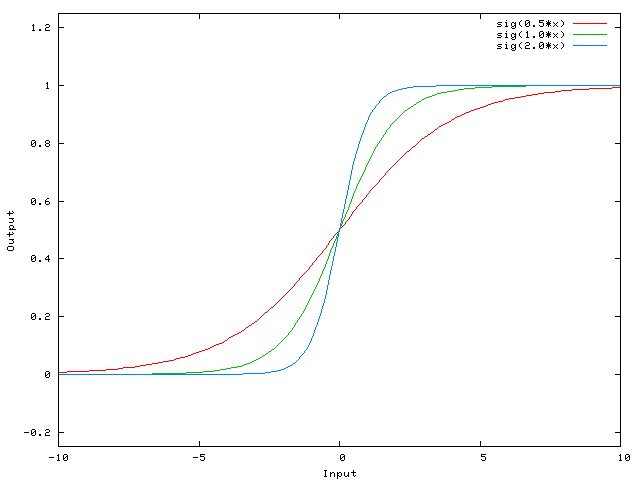
\includegraphics[scale=0.4]{images/bias.png}
        \caption{The graph of a general sigmoidal function as the coefficients (weights)
            change. A common implementation is to use functions with a range such 
            that -1 < y < 1, so assuming the network is trained to represent true with 1 
            and false with -1, this would be a great output. Pic taken from StackOverflow: http://stackoverflow.com/questions/2480650/role-of-bias-in-neural-networks}
    \end{figure}
\subsection{How Are the Correct Weights Found?}
    \paragraph{}Finding the right weights is all the work. The correct weights are found
    via a process called back propagation. Back propagation is a repeated process of error 
    correction, starting with the output nodes and moving back up the network. The error
    of the output nodes is simply the difference between the desired output and the actual
    output, but the error calculation for each node higher up the tree must be a function
    of the collective error of the exiting connections, since each node is connected to each
    node in the level down. This algorithm proved to be the most difficult part of the project
    and I consulted numerous explanations and open source projects online.\footnote{Here are some
    of the most helpful resources I found: \\  http://www.cs.montana.edu/~grayd/backprop.htm \\ http://arctrix.com/nas/python/bpnn.py}

\section{What I Would Do Differently...}
    Find a faster server

\section{Why I Used the Technologies I Did...}
    They're awesome

\section{Software Organization...}
    Submodules

\section{Hardest Part...}
    How do I do this
    \begin{lstlisting}
    class Node():
        
        def __init__(self):
            print('Making a new node')
    \end{lstlisting}

\section{Complex Data Structures and Algorithms...}
    Machine learning is hard

\section{As Hard As I Expected...}
    Machine learning is hard


\begin{center}
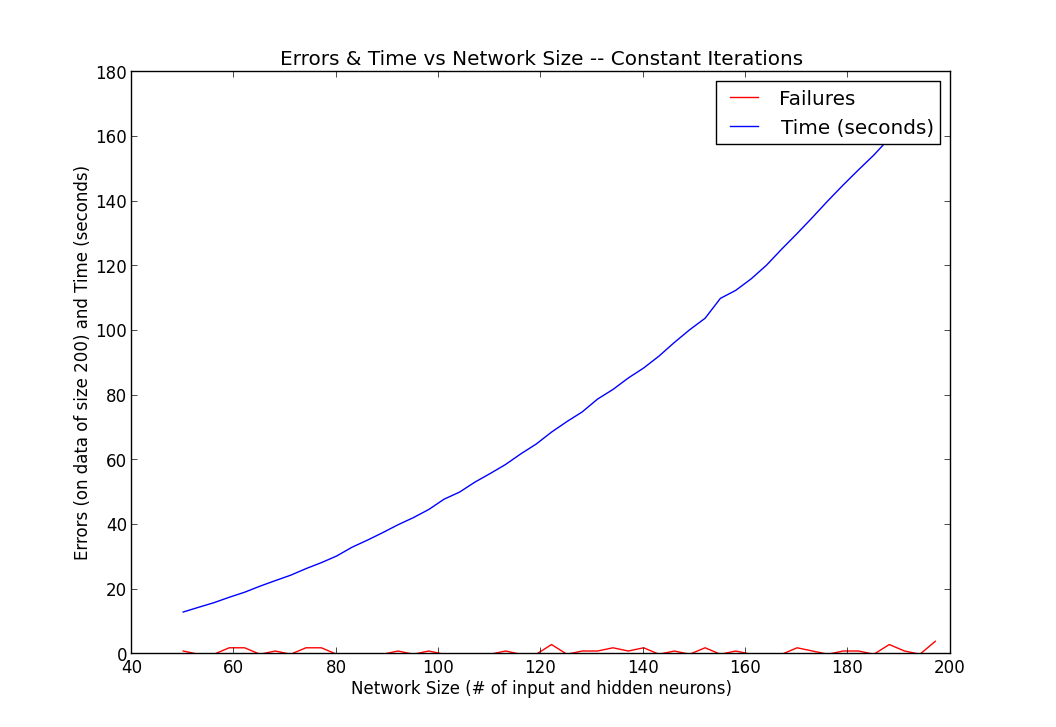
\includegraphics[scale=0.6]{good_learning.png}
\end{center}

\end{document}
